\section{Durchführung}
\label{sec:Durchführung}

\subsection{Versuchsaufbau}
Der Versuchsaufbau in in \autoref{fig:aufbau} dargestellt.\\
\begin{figure}[H]
    \centering
    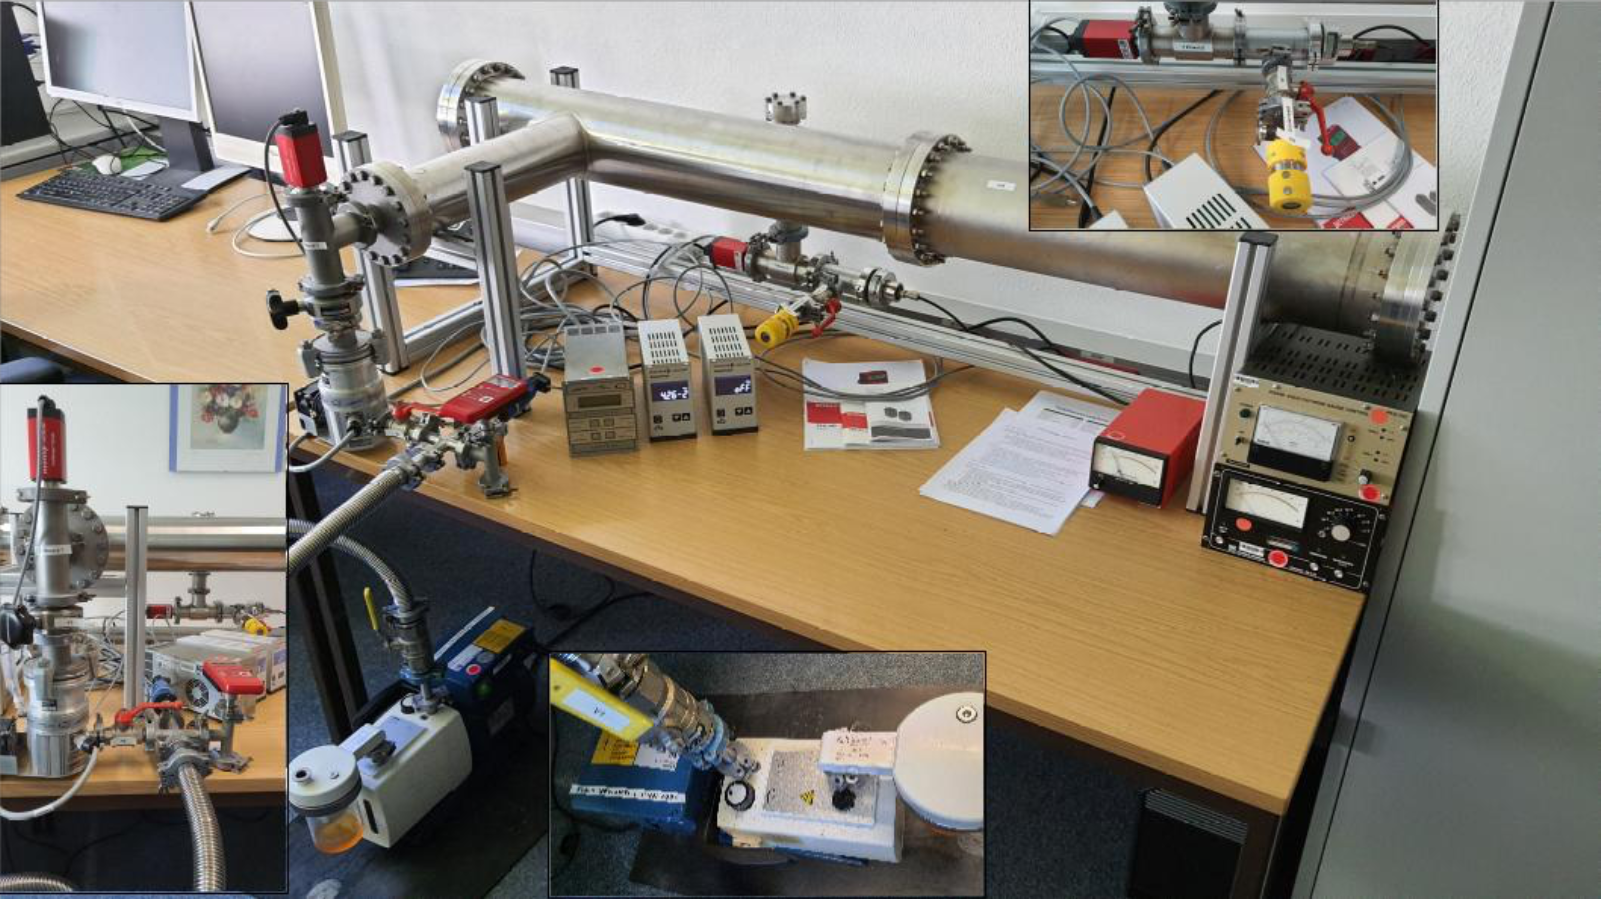
\includegraphics[width=0.8\textwidth]{content/pics/aufbau.png}
    \caption{Verschiedene Aufnahmen des Versuchsaufbaus \cite{V70}.}
    \label{fig:aufbau}
\end{figure}
Die wichtigsten Bestandteile sind die Drehschieberpumpe, die Turbomolekularpumpe und die beiden Druckmessgeräte.
Beide Pumpen können mithilfe von Ventilen abgeschiebert werden. Das gelbe Ventil (Dosierventil) erlaubt es, ein präzise dosiertes
Leck zu erzeugen.
Die Volumina des Versuchsaufbaus werden für die späteren Rechnungen benötigt und sind bekannt, mit Drehschieberpumpe
sind es $\qty{34.0+-0.1}{\liter}$ und mit Turbomolekularpumpe $\qty{33.0+-0.1}{\liter}$.
Im folgenden werden die wichtigsten Daten der verwendeten Gerätschaften aufgeführt. \cite{V70}
\begin{itemize}
    \item Drehschieberpumpe: Firma ILMVAC, Typ 300883/AKD16, Saugvermögen $\qty{4.6}{\cubic\metre\per\hour}$ bis $\qty{5.5}{\cubic\metre\per\hour}$,
    Enddruck $\qty{2e-3}{\milli\bar}$
    \item Turbomolekularpumpe: Firma ILMVAC, Typ SST81, Betriebsfrequenz $\qty{1350}{\hertz}$, Saugvermögen $\qty{77}{\liter\per\second}$
    \item Kombinierter Pirani/Kaltkathode-Sensor (2 x rote Messgeräte verbaut am Rezipienten) ausgelesen mit 2 x Anzeigegeräte TPG 361, Pfeiffer Vacuum („SingleGauge“):
    Firma Pfeiffer Vacuum, Typ PKR 360, Messbereich $\SIrange{10 e-9}{1000}{\hecto\pascal}$, Messgenauigkeit $30 \%$ des Messwertes bei
    $\SIrange{10 e-8}{100}{\hecto\pascal}$ und $50 \%$ des Messwertes bei $\SIrange{100}{1000}{\hecto\pascal}$
    \item Kombinierter Piezo/Pirani-Sensor: Firma Pfeiffer Vacuum, Typ TPG202, Messbereich $\SIrange{1200}{5 e-4}{\hecto\pascal}$,
    Messgenauigkeit $0,3 \%$ vom Vollausschlag bei $\SIrange{1200}{10}{\hecto\pascal}$, $10\%$ bei $\SIrange{10}{2 e-3}{\hecto\pascal}$
    und Faktor 2 vom Messwert bei $\leq \SI{2 e-3}{\hecto\pascal}$
\end{itemize}

\subsection{Versuchsdurchführung}
Zu Beginn wird mit der Drehschieberpumpe ein Vorvakuum von $\qty{0.1}{\milli\bar}$ erzeugt. Dannach wird die Turbomolekularpumpe hinzugeschaltet,
um ein möglichst hohes Vakuum zu erzeugen. Die Pumpe wird mindestes $\qty{30}{\minute}$ laufen gelassen, damit möglichst viele
Rückstände aus dem Aufbau entfernt werden und der Enddruck $p_{\text{E}}$ aufgenommen werden kann.
Um die Evakuierungskurve der Turbomolekularpumpe aufzunehmen, wird mithilfe des Dosierventils ein Gleichgewichtsdruck von $\qty{5e-3}{\milli\bar}$
eingestellt. Anschließend wird das Leck verschlossen und für $\qty{120}{\second}$ alle $\qty{5}{\second}$ ein Messwert für den Druck
genommen, diese Messung wird dreimal wiederholt.
Um das Saugvermögen der Turbomolekularpumpe zu bestimmen, wird eine Leckratenmessung durchgeführt. Dafür wird erneut wie zuvor
beschrieben ein Gleichgewichtsdruck eingestellt, der also eine definierte Leckrate aufweist. Nun wird die Pumpe
abgeschiebert und der Druckanstieg mit der Zeit mit den selben Messintervallen wie zuvor aufgenommen. Dieses Vorgehen wird für
drei weitere Leckraten wiederholt.\\
Die Messungen für die Drehschieberpumpe werden analog durchgeführt, nachdem die Turbomolekularpumpe ausgeschaltet wurde.
Die Evakuierungskurve wird ausgehend vom Atmosphärendruck für $\qty{600}{\second}$ in $\qty{10}{\second}$ Schritten aufgenommen.
Bei der Leckratenmessung wird der Vorgang für eine der vier Leckraten dreimal wiederholt, um eine Aussage über die
statistischen Fehler treffen zu können.
